%% source: 2023-sp-midterm_02
%% tags: [depth first search, start and finish times]
\begin{prob}
    Suppose a depth-first search (DFS) is run on the graph shown below using
    node $s$ as the source and adopting the convention that a node's neighbors
    are produced in ascending order of their label.

    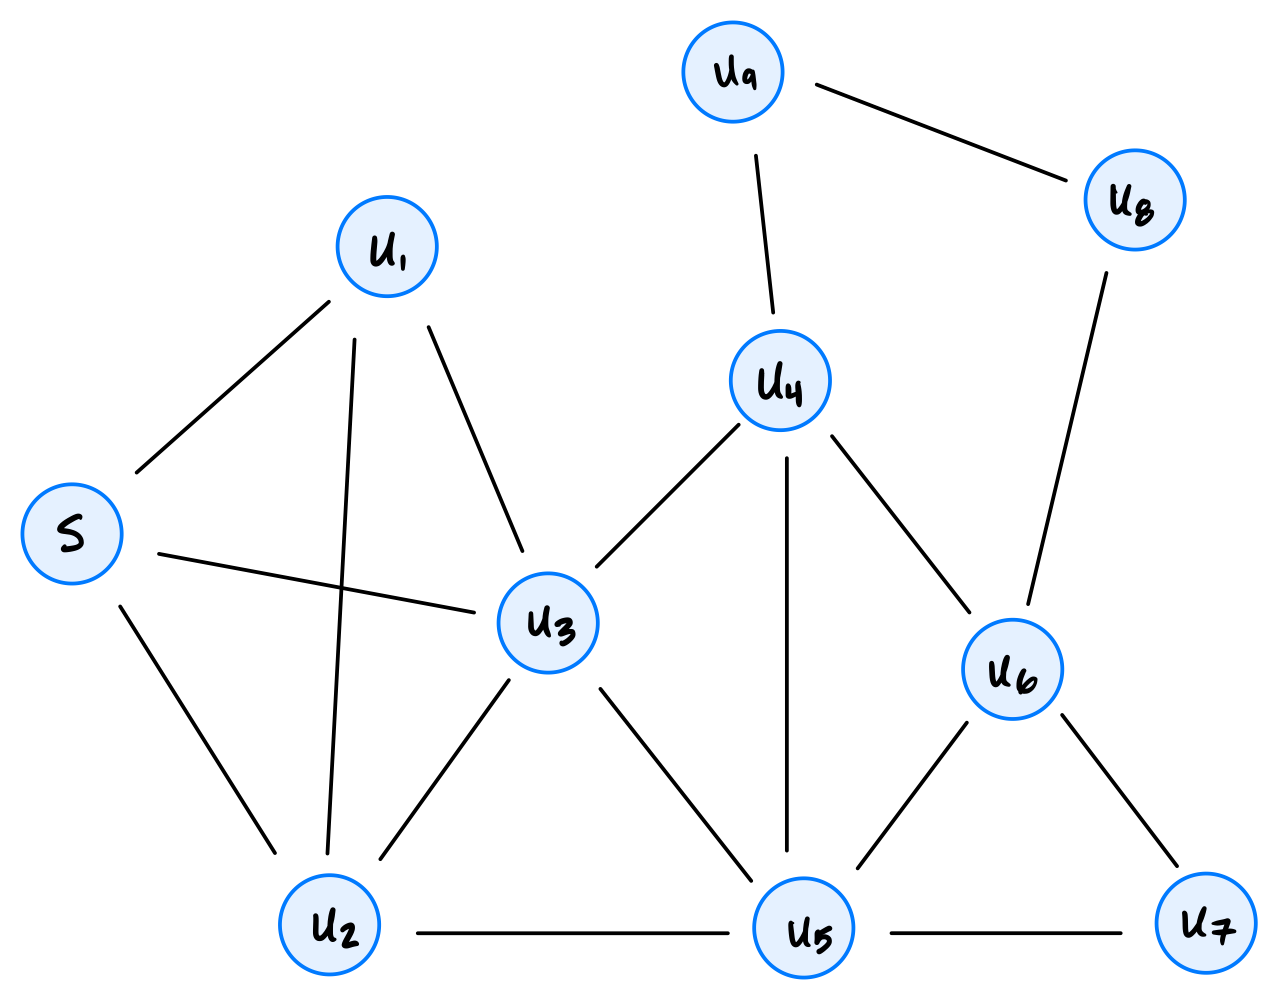
\includegraphics{./graph.png}

    \begin{subprobset}

        \begin{subprob}
            What will be the start time of node $u_7$?

            \begin{soln}
                8
            \end{soln}
        \end{subprob}

        \begin{subprob}
            What will be the finish time of node $u_7$?

            \begin{soln}
                9
            \end{soln}
        \end{subprob}

        \begin{subprob}
            Which node will be the DFS predecessor of node $u_7$?

            \begin{soln}
                $u_6$
            \end{soln}
        \end{subprob}

    \end{subprobset}


\end{prob}
